%=======================================================================
%  Slides 16-41 - Prompting: GEPA (ICLR 2026)
%=======================================================================
\section{Prompting: GEPA}

% ------------------------------------------------------------------ 16
\SectionSlide{2. GEPA}{Reflective Prompt Evolution Can Outperform RL}{%
  \small
  \begin{tabular}{@{}l@{\hspace{0.6em}}l@{}}
    \textbf{2.1} & \textbf{Bài toán}\\
    \textbf{2.2} & \textbf{Một số công trình liên quan}\\
                 & {\color{white!80}2.2.1 Prompt Opt (MIPROv2)}\\
                 & {\color{white!80}2.2.2 EvoPrompt}\\
    \textbf{2.3} & \textbf{Pipeline GEPA}\\
                 & {\color{white!80}2.3.1 Chọn lọc trên biên Pareto}\\
                 & {\color{white!80}2.3.2 Đột biến bằng Phản chiếu}\\
                 & {\color{white!80}2.3.3 System-aware Merge}\\
    \textbf{2.4} & \textbf{Kết quả thực nghiệm}\\
    \textbf{2.5} & \textbf{Giới hạn \& Tổng kết}
  \end{tabular}}

% ------------------------------------------------------------------ 17
\begin{frame}{2.1\quad Bài toán}
  \vspace{0.4em}
  \centering\DeckFig[0.78]{compound_ai}{0.88\linewidth}
\end{frame}

% ------------------------------------------------------------------ 18
\begin{frame}{2.1\quad Bài toán}
  \begin{itemize}\setlength{\itemsep}{0.8em}
    \item Hệ thống gồm $\mathbf{k}$ module LLM nối tiếp nhau.
    \item Mỗi module $i$ được điều khiển bởi prompt $\pi_i$
    \item Một ứng viên hệ thống là tập prompt: $\Phi = \{\pi_1, \pi_2, \dots, \pi_k\}$
    \item Toàn bộ trọng số mô hình gốc ($\theta$) được đóng băng $\rightarrow$ chỉ tối ưu
          trên không gian văn bản rời rạc
  \end{itemize}
\end{frame}

% ------------------------------------------------------------------ 19
\begin{frame}{2.2\quad Một số công trình liên quan}
  \Sub{2.2.1 MIPROv2 --- {\normalfont\href{https://arxiv.org/abs/2406.11695}{\color{NavySoft}\underline{https://arxiv.org/abs/2406.11695}}}}
  \vspace{0.4em}
  \begin{itemize}\setlength{\itemsep}{0.6em}
    \item \textbf{Chuẩn mực SOTA \& đối thủ so sánh trực tiếp} của GEPA trong nhánh tối ưu
          Prompt tự động (Bayesian Optimization) cho hệ thống nhiều bước (Compound AI System)
    \item Đóng băng trọng số mô hình gốc ($\theta$), chỉ tìm tổ hợp bộ chỉ dẫn (instruction)
          và ví dụ mẫu (few-shot) tối ưu
  \end{itemize}
\end{frame}

% ------------------------------------------------------------------ 20
\begin{frame}{2.2\quad Một số công trình liên quan}
  \begin{columns}[T,onlytextwidth]
    \begin{column}{0.66\textwidth}
      \Sub{2.2.1 MIPROv2 --- Cơ chế hoạt động:}
      \begin{enumerate}\setlength{\itemsep}{0.5em}
        \item \textbf{Bootstrapping:} Chạy hệ thống trên dữ liệu mẫu để thu thập các cặp ví
              dụ few-shot thành công
        \item \textbf{Grounded Proposal:} Dùng LLM sinh ra nhiều ứng viên câu chỉ dẫn dựa
              trên mô tả tác vụ và dữ liệu
        \item \textbf{Tìm kiếm tổ hợp} (Bayesian Optimization): Đánh giá trên tập validation
              để chọn tổ hợp (Instruction $+$ Few-shot) tốt nhất cho từng module
      \end{enumerate}
    \end{column}
    \begin{column}{0.31\textwidth}
      \centering\vspace{-0.3em}\DeckFig[0.74]{miprov2}{\linewidth}
    \end{column}
  \end{columns}
\end{frame}

% ------------------------------------------------------------------ 21
\begin{frame}{2.2\quad Một số công trình liên quan}
  \Sub{2.2.1 MIPROv2 --- Hạn chế:}
  \vspace{0.3em}
  \begin{itemize}\setlength{\itemsep}{0.7em}
    \item Vẫn dựa chủ yếu vào điểm số tổng (scalar metric)\\
          $\rightarrow$ bỏ phí thông tin chẩn đoán từ dấu vết lỗi sai (execution traces)
    \item Có xu hướng nhồi nhiều ví dụ few-shot để kéo điểm\\
          $\rightarrow$ prompt sinh ra rất dài, làm đội Inference Token Budget và tăng độ
          trễ suy luận
  \end{itemize}
\end{frame}

% ------------------------------------------------------------------ 22
\begin{frame}{2.2\quad Một số công trình liên quan}
  \Sub{2.2.2 EvoPrompt --- {\normalfont\href{https://arxiv.org/abs/2309.08532}{\color{NavySoft}\underline{https://arxiv.org/abs/2309.08532}}}}
  \vspace{0.4em}
  \begin{itemize}\setlength{\itemsep}{0.6em}
    \item \textbf{Tiền đề (Motivation)} cho khung tiến hóa của GEPA: kết hợp
          \textbf{Thuật toán tiến hóa} với LLM để tối ưu prompt tự động
    \item Duy trì một quần thể nhiều prompt ứng viên qua các thế hệ
    \item Ở mỗi vòng lặp: chọn các prompt có điểm đánh giá cao, dùng LLM thực hiện
          \textbf{Đột biến} và \textbf{Lai ghép} để sinh prompt mới
  \end{itemize}
\end{frame}

% ------------------------------------------------------------------ 23
\begin{frame}{2.2\quad Một số công trình liên quan}
  \Sub{2.2.2 EvoPrompt --- Hạn chế:}
  \vspace{0.3em}
  \begin{itemize}\setlength{\itemsep}{0.65em}
    \item \textbf{Đột biến ``mù quáng'':} Chỉ sửa câu chữ ngẫu nhiên dựa trên điểm số, không
          biết prompt sai ở bước nào $\rightarrow$ thử sai tốn kém, hội tụ chậm
    \item \textbf{Chọn lọc theo điểm trung bình:} Dễ làm mất sự đa dạng và bị kẹt ở cực trị
          địa phương
    \item \textbf{Chỉ tối ưu 1 prompt đơn lẻ:} Khó mở rộng sang hệ thống nhiều prompt (module)
          nối tiếp nhau (\textbf{Compound AI System})
  \end{itemize}
  \vspace{0.4em}
  \begin{beamercolorbox}[wd=\linewidth,sep=0.55em]{block body}
    $\Rightarrow$ \textbf{Động lực của GEPA:} Giữ khung tiến hóa nhưng nâng cấp bằng
    \textbf{Đột biến Phản chiếu}, \textbf{Biên Pareto} và \textbf{Lai ghép theo cấu trúc (LCA)}.
  \end{beamercolorbox}
\end{frame}

% ------------------------------------------------------------------ 24
\begin{frame}{2.3\quad GEPA}
  \Sub{Thiết lập dữ liệu}
  \begin{itemize}\setlength{\itemsep}{0.45em}
    \item \textbf{Chia tập $D_{\text{train}}$ thành 2 phần tách biệt}:
      \begin{itemize}\tightlist
        \item $D_{\text{feedback}}$ \textit{(như tập Train)}: Nguồn bốc mẫu cho phần đột biến
              prompt soi lỗi và sửa prompt.
        \item $D_{\text{pareto}}$ \textit{(như Validation nội bộ)}: Tập cố định (vài chục đến
              $\sim$100 mẫu), dùng để chấm điểm như tập validation.
      \end{itemize}
    \item \textbf{Minibatch ($\mathcal{M}$):} Nhóm nhỏ cố định ($b \approx 3$--$5$ mẫu) bốc ngẫu
          nhiên từ $D_{\text{feedback}}$ mỗi vòng $\rightarrow$ vừa đủ ngắn để đọc kỹ lỗi,
          vừa làm vòng loại nhanh.
  \end{itemize}
\end{frame}

% ------------------------------------------------------------------ 25
\begin{frame}{2.3\quad GEPA}
  \Sub{Khái niệm cốt lõi}
  \begin{itemize}\setlength{\itemsep}{0.4em}
    \item \textbf{Prompt khởi tạo ($P_0$):} Bộ prompt cơ bản ban đầu cho $k$ module (viết tay
          ngắn gọn hoặc prompt zero-shot mặc định của framework). \textbf{Không} cần tối ưu
          sẵn --- chỉ cần đúng định dạng để hệ thống chạy được và sinh traces.
    \item \textbf{Candidate Pool ($\mathcal{P}$):} Kho lưu trữ dạng \textbf{cây tiến hóa}
          (gốc là $P_0$), lưu mọi ứng viên vượt qua vòng lọc minibatch kèm bảng điểm trên
          $D_{\text{pareto}}$ và quan hệ cha--con (phục vụ lọc Pareto \& Merge).
    \item \textbf{Rollout:} 1 lượt chạy hoàn chỉnh hệ thống AI trên 1 mẫu dữ liệu.
    \item \textbf{Rollout Budget ($B$):} Siêu tham số giới hạn tổng số lượt Rollout tối đa
          (\texttt{While Budget > 0}); hết ngân sách thì dừng và chọn ứng viên điểm trung bình
          cao nhất trên $D_{\text{pareto}}$.
  \end{itemize}
\end{frame}

% ------------------------------------------------------------------ 26
\begin{frame}{2.3\quad GEPA}
  \centering\DeckFig[0.9]{gepa_flow_vi}{\linewidth}
\end{frame}

% ------------------------------------------------------------------ 27
\begin{frame}{2.3\quad GEPA}
  \centering
  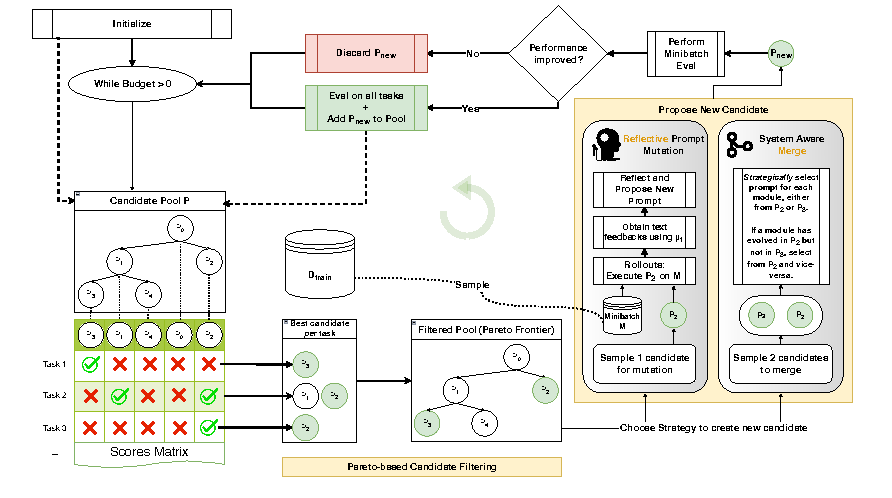
\includegraphics[width=\linewidth,height=0.9\textheight,keepaspectratio]{figure/gepa/fig3_pipeline}
\end{frame}

% ------------------------------------------------------------------ 28
\begin{frame}{2.3\quad GEPA}
  \Sub{2.3.1 Thuật toán: Chọn lọc trên biên Pareto}
  \begin{itemize}\setlength{\itemsep}{0.35em}
    \item Chỉ giữ 1 ứng viên có điểm trung bình cao nhất\\
          $\rightarrow$ dễ mất đa dạng chiến lược và kẹt ở cực trị địa phương
    \item Với mỗi mẫu dữ liệu $x_j \in D_{\text{pareto}}$, tìm điểm số cao nhất mà quần
          thể $\mathcal{P}$ đạt được:
          \[ s^*(x_j) = \max_{\Phi\in\mathcal{P}} s(\Phi, x_j) \]
    \item Chỉ giữ lại các ứng viên đạt đỉnh $s^*(x_j)$ trên ít nhất một mẫu $x_j$ (loại
          bỏ ứng viên bị thống trị hoàn toàn --- dominated)
    \item Xác suất chọn ứng viên $\Phi$: Tỷ lệ thuận với số lượng mẫu $x_j$ mà $\Phi$ đạt
          điểm cao nhất
  \end{itemize}
\end{frame}

% ------------------------------------------------------------------ 29
\begin{frame}{2.3\quad GEPA}
  \Sub{2.3.1 Thuật toán: Chọn lọc trên biên Pareto}
  \centering\DeckFig[0.64]{pareto_filter}{0.92\linewidth}
\end{frame}

% ------------------------------------------------------------------ 30
\begin{frame}{2.3\quad GEPA}
  \begin{columns}[T,onlytextwidth]
    \begin{column}{0.5\textwidth}
      \Sub{2.3.1 Chọn lọc trên biên Pareto}
      \vspace{0.4em}
      \textbf{Ý nghĩa:}
      \begin{itemize}\setlength{\itemsep}{0.6em}
        \item Giữ lại đồng thời các ``chuyên gia'' giải tốt những dạng bài con khác nhau
        \item Cân bằng giữa \textbf{khai thác} (ứng viên giỏi nhiều mẫu) và \textbf{khám
              phá} (ứng viên giỏi các ca khó/ngách)
      \end{itemize}
    \end{column}
    \begin{column}{0.47\textwidth}
      \centering\DeckFig[0.74]{algo2_pareto}{\linewidth}
    \end{column}
  \end{columns}
\end{frame}

% ------------------------------------------------------------------ 31
\begin{frame}{2.3\quad GEPA}
  \Sub{2.3.2 Reflective Prompt Mutation}
  \vspace{0.6em}
  \begin{beamercolorbox}[wd=\linewidth,sep=0.7em]{block body}
    \textbf{Mục tiêu:} Sửa lỗi có chủ đích cho từng module dựa trên dấu vết thực thi
    (thay vì sửa ngẫu nhiên như EvoPrompt).
  \end{beamercolorbox}
\end{frame}

% ------------------------------------------------------------------ 32
\begin{frame}{2.3\quad GEPA}
  \Sub{2.3.2 Reflective Prompt Mutation}
  \begin{itemize}\setlength{\itemsep}{0.3em}
    \item \textbf{Chọn module ($\pi_i$):} Chọn 1 module trong ứng viên $\Phi$ (xoay vòng
          Round-Robin)
    \item \textbf{Chạy thử:} Chạy $\Phi$ trên minibatch $\mathcal{M}$ $\rightarrow$ thu thập
          Execution Traces và phản hồi lỗi ($f$) qua hàm $\mu_f$
    \item \textbf{Phản chiếu (Reflection LM):} Dùng LLM thông thường qua Meta-Prompt đọc
          ($\pi_i$ cũ $+$ Traces $+$ Feedback $f$) $\rightarrow$ chẩn đoán nguyên nhân và viết
          lại $\pi_i$ mới cô đọng, có quy tắc rõ ràng
    \item \textbf{Màng lọc Eval 2 tầng:} Chạy thử $\Phi_{\text{new}}$ trên chính minibatch
          $\mathcal{M}$:
      \begin{itemize}\tightlist
        \item Điểm KHÔNG tăng $\rightarrow$ \textbf{Discard} ngay để tiết kiệm Rollout Budget.
        \item Điểm TĂNG $\rightarrow$ Chấm \textbf{Eval on all tasks} ($D_{\text{pareto}}$)
              và thêm vào quần thể $\mathcal{P}$.
      \end{itemize}
  \end{itemize}
\end{frame}

% ------------------------------------------------------------------ 33
\begin{frame}{2.3\quad GEPA}
  \Sub{2.3.3 System-aware Merge (LCA)}
  \begin{itemize}\setlength{\itemsep}{0.45em}
    \item \textbf{Khi nào kích hoạt?} Sau khi một vòng Đột biến thành công (giới hạn mặc định
          \texttt{max\_merge = 5}), nếu trên Biên Pareto có $\ge 2$ ứng viên thuộc các nhánh
          khác nhau chưa từng ghép
    \item \textbf{Cơ chế ghép theo Tổ tiên chung gần nhất (LCA):}
      \begin{itemize}\tightlist
        \item So sánh từng module của 2 nhánh ($P_A, P_B$) với bản gốc chung $P_{\text{LCA}}$.
        \item Nhánh nào đã nâng cấp module $i$ thì lấy module đó; nếu cả 2 cùng sửa 1 module
              $\rightarrow$ ưu tiên nhánh có điểm tổng cao hơn.
      \end{itemize}
    \item \textbf{Kiểm tra nhanh:} Không tốn lệnh gọi Reflection LM; chạy thử bản ghép
          $P_{\text{merge}}$ trên minibatch $\rightarrow$ nếu không tụt điểm so với $P_A, P_B$
          thì chấm trên $D_{\text{pareto}}$ và thêm vào Pool
  \end{itemize}
\end{frame}

% ------------------------------------------------------------------ 34
\begin{frame}{2.3\quad GEPA}
  \Sub{2.3.3 System-aware Merge}
  \centering
  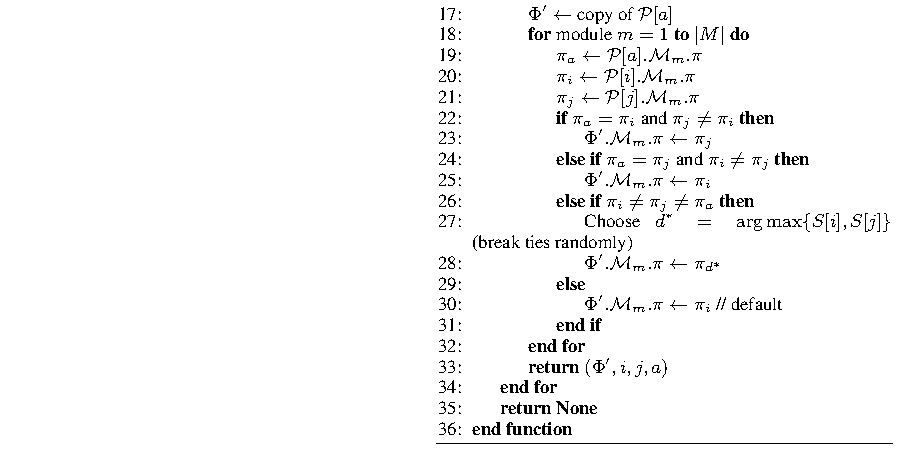
\includegraphics[width=\linewidth,height=0.6\textheight,keepaspectratio]{figure/gepa/fig9_merge}
  \par\vspace{0.2em}{\color{Muted}\scriptsize Hình 9 --- GEPA (ICLR 2026)}
\end{frame}

%=======================================================================
%  Slides 35-39 - 2.4 Kết quả thực nghiệm (Experiments)
%=======================================================================

% ------------------------------------------------------------------ 35
\begin{frame}{2.4\quad Kết quả thực nghiệm}
  \Sub{Thiết lập thực nghiệm (Experimental Setup)}
  \begin{itemize}\setlength{\itemsep}{0.55em}
    \item \textbf{Mô hình đánh giá (2 nhóm):}
      \begin{itemize}\tightlist
        \item Mã nguồn mở: \textbf{Qwen3 8B} (cho phép chạy cả RL và Prompt Opt).
        \item Đóng (Proprietary API): \textbf{GPT-4.1 mini}.
      \end{itemize}
    \item \textbf{4 Benchmark cho Compound AI System:}
      \begin{itemize}\tightlist
        \item \textbf{HotpotQA:} Hỏi--đáp đa bước (multi-hop QA).
        \item \textbf{IFBench:} Tuân thủ chỉ dẫn phức tạp (instruction following).
        \item \textbf{HoVer:} Kiểm chứng thông tin đa bước (fact verification).
        \item \textbf{PUPA:} Ủy quyền bảo mật quyền riêng tư (privacy-preserving delegation).
      \end{itemize}
    \item \textbf{Đối thủ so sánh (Baselines):} Baseline gốc ($P_0$), \textbf{GRPO} (RL SOTA
          trên Qwen3 8B), \textbf{MIPROv2} (Prompt Opt SOTA), và 2 cấu hình \textbf{GEPA} /
          \textbf{GEPA+Merge}.
  \end{itemize}
\end{frame}

% ------------------------------------------------------------------ 36
\begin{frame}{2.4\quad Kết quả thực nghiệm}
  \Sub{Observation 1: Vượt trội GRPO (RL) với số Rollout ít hơn tới $35\times$}
  \begin{columns}[T,onlytextwidth]
    \begin{column}{0.44\textwidth}
      \begin{itemize}\setlength{\itemsep}{0.55em}
        \item Trên \textbf{Qwen3 8B}, GEPA vượt \textbf{GRPO} trên toàn bộ 4 benchmark
              (trung bình cao hơn $\sim$10\%, có tác vụ tới $\sim$20\%)
        \item \textbf{Hiệu quả mẫu vượt trội:} GRPO cần tới $\sim$24.000 rollouts, trong
              khi GEPA chỉ cần vài trăm đến $\sim$1.200 rollouts (tiết kiệm tới
              \textbf{$35\times$})
        \item \textbf{Lý do:} Học từ phản hồi ngôn ngữ giàu thông tin thay vì chỉ điểm
              thưởng vô hướng
      \end{itemize}
    \end{column}
    \begin{column}{0.53\textwidth}
      \centering
      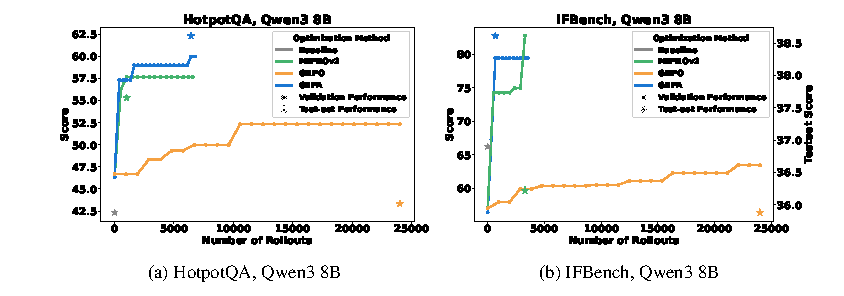
\includegraphics[width=\linewidth,height=0.68\textheight,keepaspectratio]{figure/gepa/fig_obs1_grpo_rollouts}
      \par\vspace{0.2em}{\color{Muted}\scriptsize Biểu đồ Score theo Rollout Budget --- GEPA (ICLR 2026)}
    \end{column}
  \end{columns}
\end{frame}

% ------------------------------------------------------------------ 37
\begin{frame}{2.4\quad Kết quả thực nghiệm}
  \Sub{Observation 2: Vượt trội MIPROv2 trên cả mô hình Mở \& Đóng}
  \begin{columns}[T,onlytextwidth]
    \begin{column}{0.44\textwidth}
      \begin{itemize}\setlength{\itemsep}{0.55em}
        \item GEPA vượt \textbf{MIPROv2} trên tất cả benchmark ở cả \textbf{Qwen3 8B}
              lẫn \textbf{GPT-4.1 mini} (trung bình cao hơn $>10\%$)
        \item Chứng minh \textbf{Đột biến Phản chiếu $+$ Biên Pareto} hiệu quả hơn hẳn
              tìm kiếm tổ hợp Bayesian dựa trên điểm số tổng
        \item Hiệu quả ổn định ngay cả khi không thể cập nhật trọng số mô hình (API đóng)
      \end{itemize}
    \end{column}
    \begin{column}{0.53\textwidth}
      \centering
      % FIGURE PLACEHOLDER (chua co file): figure/gepa/fig_obs2_main_table
      % \includegraphics[width=\linewidth,height=0.68\textheight,keepaspectratio]{figure/gepa/fig_obs2_main_table}
      \par\vspace{0.2em}{\color{Muted}\scriptsize Bảng/Biểu đồ so sánh tổng thể --- GEPA (ICLR 2026)}
    \end{column}
  \end{columns}
\end{frame}

% ------------------------------------------------------------------ 38
\begin{frame}{2.4\quad Kết quả thực nghiệm}
  \Sub{Observation 3: Prompt ngắn gọn hơn $\rightarrow$ Tiết kiệm Inference Token Budget}
  \begin{columns}[T,onlytextwidth]
    \begin{column}{0.46\textwidth}
      \begin{itemize}\setlength{\itemsep}{0.55em}
        \item \textbf{MIPROv2} có xu hướng nhồi nhiều ví dụ \textit{few-shot} để kéo điểm
              $\rightarrow$ prompt rất dài
        \item \textbf{GEPA} tổng hợp lỗi sai thành các \textbf{quy tắc cô đọng}
              $\rightarrow$ độ dài prompt ngắn hơn tới \textbf{$9\times$} so với MIPROv2
        \item Giúp giảm mạnh \textbf{chi phí suy luận (Inference Token Budget)} và độ trễ
              khi triển khai thực tế
      \end{itemize}
    \end{column}
    \begin{column}{0.51\textwidth}
      \centering
      % FIGURE PLACEHOLDER (chua co file): figure/gepa/fig_obs3_prompt_length
      % \includegraphics[width=\linewidth,height=0.68\textheight,keepaspectratio]{figure/gepa/fig_obs3_prompt_length}
      \par\vspace{0.2em}{\color{Muted}\scriptsize So sánh độ dài Prompt / Chi phí suy luận --- GEPA (ICLR 2026)}
    \end{column}
  \end{columns}
\end{frame}

% ------------------------------------------------------------------ 39
\begin{frame}{2.4\quad Kết quả thực nghiệm}
  \Sub{Observation 4: Tác động của Biên Pareto \& System-aware Merge}
  \begin{columns}[T,onlytextwidth]
    \begin{column}{0.46\textwidth}
      \begin{itemize}\setlength{\itemsep}{0.55em}
        \item \textbf{Biên Pareto vs. Tham lam (Greedy):} Chọn lọc Pareto luôn cho điểm
              cao và ổn định hơn nhờ giữ đa dạng chiến lược, tránh kẹt cực trị địa phương
        \item \textbf{System-aware Merge (LCA):}
          \begin{itemize}\tightlist
            \item Trên mô hình mạnh (\textbf{GPT-4.1 mini}): \texttt{GEPA+Merge} giúp cộng
                  thêm $\sim$5\% điểm so với \texttt{GEPA} thường.
            \item Trên mô hình nhỏ (\textbf{Qwen3 8B}): nhạy cảm với thời điểm ghép; ghép
                  quá sớm đôi khi làm điểm trung bình hơi giảm.
          \end{itemize}
      \end{itemize}
    \end{column}
    \begin{column}{0.51\textwidth}
      \centering
      % FIGURE PLACEHOLDER (chua co file): figure/gepa/fig_obs4_ablation
      % \includegraphics[width=\linewidth,height=0.68\textheight,keepaspectratio]{figure/gepa/fig_obs4_ablation}
      \par\vspace{0.2em}{\color{Muted}\scriptsize Kết quả Ablation (Pareto / Merge) --- GEPA (ICLR 2026)}
    \end{column}
  \end{columns}
\end{frame}

%=======================================================================
%  Slides 40-41 - 2.5 Giới hạn & Tổng kết
%=======================================================================

% ------------------------------------------------------------------ 40
\begin{frame}{2.5\quad Giới hạn \& Tổng kết}
  \Sub{Giới hạn của GEPA}
  \begin{itemize}\setlength{\itemsep}{0.6em}
    \item \textbf{Phụ thuộc vào Reflection LM \& chất lượng phản hồi ($\mu_f$):}\\
          Cần một LLM đủ mạnh để chẩn đoán đúng nguyên nhân gốc rễ; hiệu quả sẽ giảm nếu
          bài toán chỉ có điểm số thô mà không có dấu vết thực thi (traces) hoặc phản hồi
          lỗi rõ ràng.
    \item \textbf{Độ nhạy của System-aware Merge:}\\
          Hiệu quả ghép nhánh phụ thuộc vào năng lực mô hình và thời điểm kích hoạt (tăng
          mạnh trên GPT-4.1 mini nhưng dễ làm tụt nhẹ điểm trên mô hình nhỏ như Qwen3 8B
          nếu ghép quá sớm).
    \item \textbf{Giới hạn trần của việc đóng băng trọng số ($\theta$):}\\
          Chỉ tối ưu trên không gian văn bản nên khó giải quyết các tác vụ đòi hỏi nạp tri
          thức chuyên ngành hoàn toàn mới hoặc vượt quá năng lực suy luận sẵn có của mô hình
          gốc.
  \end{itemize}
\end{frame}

% ------------------------------------------------------------------ 41
\begin{frame}{2.5\quad Giới hạn \& Tổng kết}
  \Sub{Tổng kết (Key Takeaways)}
  \begin{itemize}\setlength{\itemsep}{0.55em}
    \item \textbf{Phản hồi ngôn ngữ $>$ Điểm thưởng vô hướng:} Khai thác Execution Traces
          qua Đột biến Phản chiếu giúp vượt trội RL (GRPO) với số lượt Rollout ít hơn tới
          \textbf{$35\times$}.
    \item \textbf{Tiến hóa cho hệ thống đa module:} Kết hợp \textbf{Biên Pareto} (giữ đa
          dạng chiến lược, chống overfit) và \textbf{System-aware Merge (LCA)} giúp tối ưu
          hiệu quả Compound AI System.
    \item \textbf{Tối ưu chi phí triển khai:} Sinh ra prompt ngắn gọn (ngắn hơn tới
          \textbf{$9\times$} so với MIPROv2), giảm mạnh \textit{Inference Token Budget} và
          áp dụng được cho cả API mô hình đóng.
  \end{itemize}
  \vspace{0.35em}
  \begin{beamercolorbox}[wd=\linewidth,sep=0.55em]{block body}
    \textbf{Mở rộng:} Khi tối ưu Prompt chạm trần do trọng số bị đóng băng $\rightarrow$
    cần chuyển sang hướng thích nghi tham số hiệu quả (\textbf{PEFT / Text-to-LoRA}).
  \end{beamercolorbox}
\end{frame}